\documentclass{article}
\usepackage{amsmath}
\usepackage{graphicx}
\usepackage{booktabs}

\title{My first document}
%\date{}
\author{Mo Khan}

\begin{document}
  \pagenumbering{gobble}
  \maketitle
  \newpage
  \tableofcontents
  \newpage
  \pagenumbering{arabic}

  \section{Section}

  Hello World!

  \subsection{Subsection}

  Structuring a document is easy!

  \subsubsection{Subsubsection}

  More text.

  \paragraph{Paragraph}

  Some more text.

  \subparagraph{Subparagraph}

  Even more text.

  \newpage
  \section{Another section}

  \begin{equation*}
    f(x) = x^2
  \end{equation*}

  This is some example text\footnote{\label{myfootnote}Hello footnote}.

  \begin{figure}[h!]
    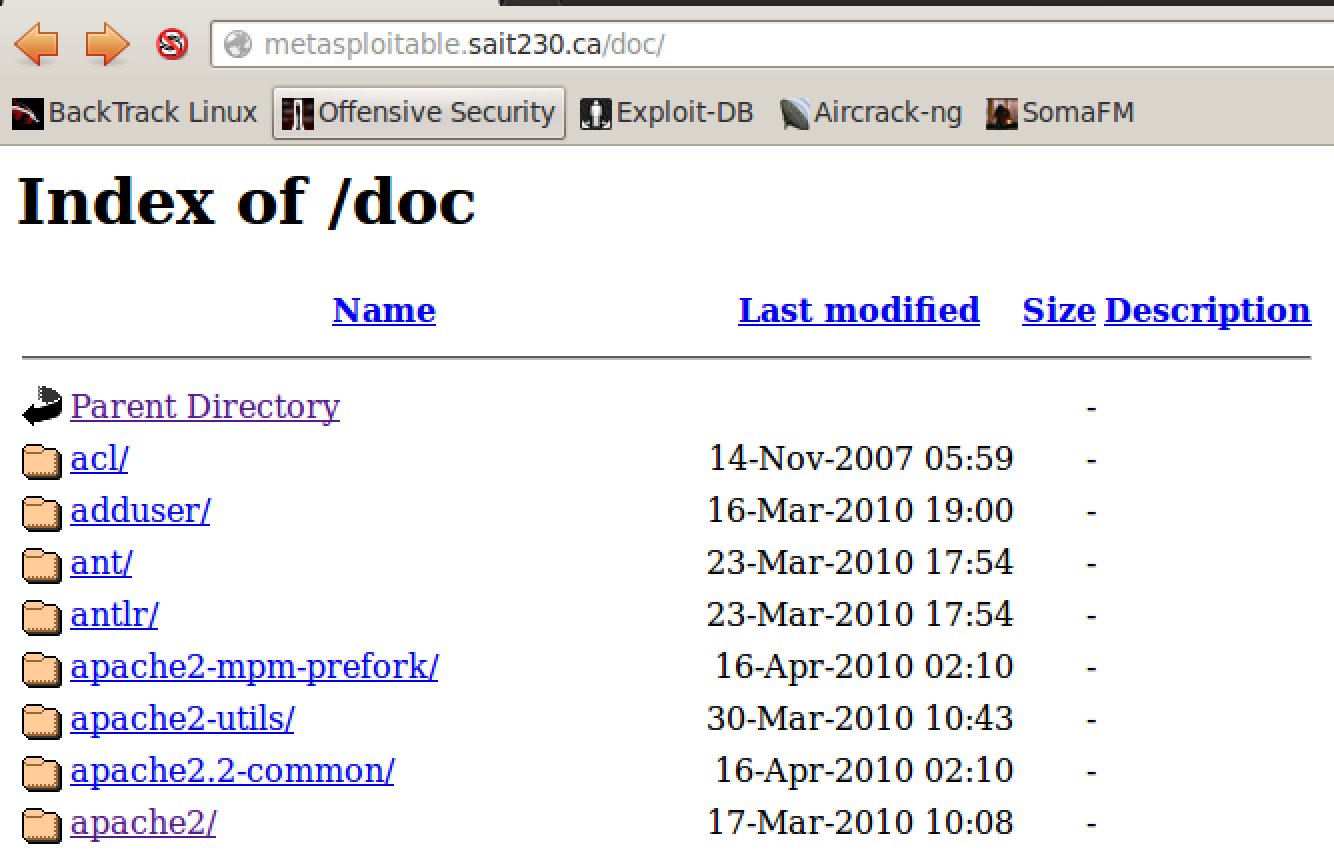
\includegraphics[width=\linewidth]{images/screenshot.png}
    \caption{A boat.}
    \label{fig:boat1}
  \end{figure}

  Figure \ref{fig:boat1} shows a boat.

  \begin{table}[h!]
    \centering
    \caption{Caption for the table.}
    \label{tab:table1}
    \begin{tabular}{l|c||r}
      1 & 2 & 3\\
      \hline
      a & b & c\\
    \end{tabular}
  \end{table}

  I'm referring to footnote \ref{myfootnote}.

  \begin{table}[h!]
    \centering
    \caption{Caption for the table.}
    \label{tab:table2}
    \begin{tabular}{ccc}
      \toprule
      Some & actual & content\\
      \midrule
      prettifies & the & content\\
      as & well & as\\
      using & the & booktabs package\\
      \bottomrule
    \end{tabular}
  \end{table}

  \newpage
  \begin{table}
    \caption{Dummy table}
  \end{table}

  \begin{appendix}
    \listoffigures
    \listoftables
  \end{appendix}

\end{document}
